% Created 2022-05-10 Tue 16:43
% Intended LaTeX compiler: xelatex
\documentclass[11pt]{article}
\usepackage{graphicx}
\usepackage{longtable}
\usepackage{wrapfig}
\usepackage{rotating}
\usepackage[normalem]{ulem}
\usepackage{amsmath}
\usepackage{amssymb}
\usepackage{capt-of}
\usepackage{hyperref}
\usepackage{color}
\usepackage{listings}
\usepackage[newfloat]{minted}
\usepackage[utf8]{inputenc}
\usepackage[table,xcdraw]{xcolor}
\usepackage{paralist}
\usepackage{datetime2}
\usepackage{graphicx}
\usepackage{lscape}
\usepackage{longtable}
\usepackage{hyperref}
\usepackage[a4paper, left=3cm, right=3cm, top=2cm]{geometry}
\usepackage{fancyhdr}
\usepackage{listings}
\usepackage{textcomp}
\usepackage{enumitem}
\usepackage{algorithm}
\usepackage{algpseudocode}
\setlist{noitemsep}
\setlength{\columnseprule}{0.2pt}
\definecolor{mygreen}{rgb}{0,0.6,0}
\definecolor{mygray}{rgb}{0.5,0.5,0.5}
\definecolor{mymauve}{rgb}{0.58,0,0.82}
\lstset{ backgroundcolor=\color{white}, basicstyle=\footnotesize, breaklines=true, captionpos=b, commentstyle=\color{mygreen}, escapeinside={\%*}{*)},keywordstyle=\color{blue}, stringstyle=\color{mymauve},}
\author{Olivier Lischer}
\date{\today}
\title{Design Patterns - Summary}
\hypersetup{
 pdfauthor={Olivier Lischer},
 pdftitle={Design Patterns - Summary},
 pdfkeywords={},
 pdfsubject={},
 pdfcreator={Emacs 27.2 (Org mode 9.5.2)}, 
 pdflang={English}}
\begin{document}

\pagestyle{fancy}
\fancyhf{}
\fancyhead[R]{SEP2-FS}
\fancyhead[L]{Design Patterns - Summary}
\fancyfoot[CE,CO]{\leftmark}
\fancyfoot[R]{\thepage}
\fancyfoot[L]{Olivier Lischer}

\begin{titlepage}
  \begin{center}
    {\Huge Design Patterns - Summary} \\
    \vspace{8 cm}

    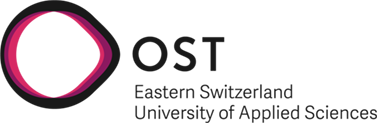
\includegraphics[height=4cm]{./img/ost-logo.png}

    \vspace{4 cm}
    Semester: Spring 2022
    \vspace{1 cm}

    Version: 0.1.0 \\
    Date: \DTMnow \\
    \vspace{3 cm}
    School of Computer Science\\
    OST Eastern Switzerland University of Applied Sciences
  \end{center}
\end{titlepage}
\newpage
\tableofcontents
\newpage


\section{Introduction}
\label{sec:org8e2a47a}
\subsection{Most important quotes}
\label{sec:org3fd2b32}
In the introduction the basics of object-oriented programming are explained.
Therefore, for many this is easy to read.
However, some important statements are made.

\begin{quote}
Favor object composition over class inheritance
\end{quote}

Because it is very difficult to make the correct abstraction often the base class(es) are not complete or have too much in it.
With object composition you don't have this problem.

\begin{quote}
Program to an interface, not an implementation
\end{quote}
If you implement against interfaces you can test your class with unit tests.
If you implement against a fixed implementation you can not change this behavior at anytime.

\subsection{The design patterns}
\label{sec:org183572f}

Class Design Patterns deal with the relationships between classes and their subclasses.
The Object Design Patterns with the object relationships which can be changed at runtime.

\begin{figure}[htbp]
\centering
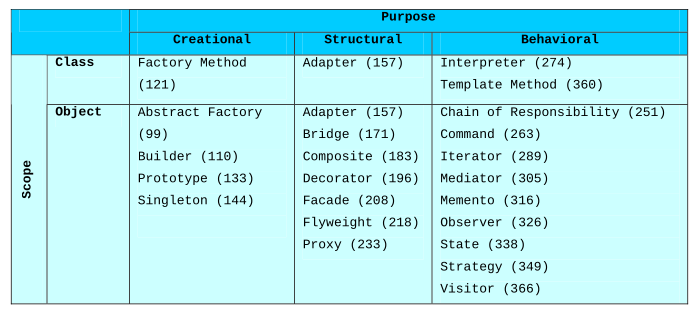
\includegraphics[width=.9\linewidth]{img/design_pattern_space.png}
\caption{\label{fig:design-pattern-space}Design pattern space}
\end{figure}


\section{Creational}
\label{sec:org9bf6940}
\subsection{Abstract Factory}
\label{sec:org0c3769f}
The Abstract Factory provides an interface for creating families of related or dependent objects without specifying their concrete class.
It is a good choice, when you want to create big class hierarchy from a factory.
In general the Simple Factory (\href{../../../../roam/20220510160458-design_pattern_simple_factory.org}{Design Pattern - Simple Factory}) is more common today.


Motivation:
\begin{itemize}
\item You want to create concrete objects without knowing which concrete type you get.
\item You are only interested in the interface.
\end{itemize}


\begin{figure}[htbp]
\centering
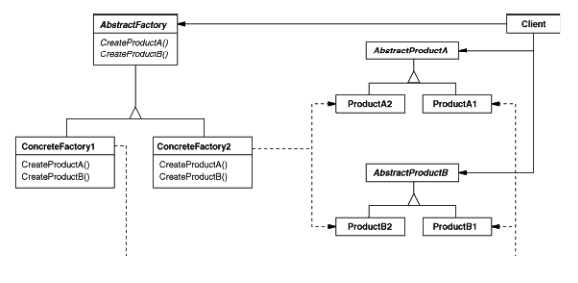
\includegraphics[width=.9\linewidth]{img/abstract_factory.png}
\caption{\label{fig:abstract-factory-uml}Abstract Factory Class Diagram}
\end{figure}

\subsubsection{Important Notes}
\label{sec:orga7071df}
The Factory must be created at the very beginning of the application.
After creation only this factory must be used to create objects.
Otherwise, the benefit of the factory are gone.

\subsection{Builder}
\label{sec:orgf8152a3}
The Builder Pattern seperates the construction of a complex class from its representation.
Therby you can hidde the creation of complex objects behind functions (see listening \ref{lst:the-builder-pattern-in-action}).


\begin{figure}[htbp]
\centering
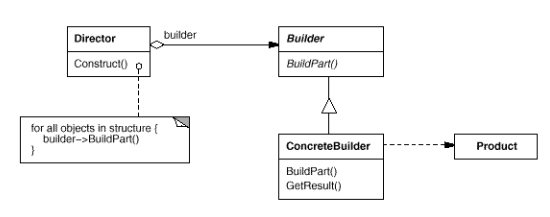
\includegraphics[width=.9\linewidth]{img/builder.png}
\caption{\label{fig:builder-class-diagram}Builder Class Diagram}
\end{figure}


\lstset{language=c++,label=lst:the-builder-pattern-in-action,caption={The Builder Pattern in Action},captionpos=b,numbers=none}
\begin{lstlisting}
Maze* MazeGame::CreateMaze () {
  Maze* aMaze = new Maze;
  Room* r1 = new Room(1);
  Room* r2 = new Room(2);
  Door* theDoor = new Door(r1, r2);
  aMaze->AddRoom(r1);
  aMaze->AddRoom(r2);
  r1->SetSide(North, new Wall);
  r1->SetSide(East, theDoor);
  r1->SetSide(South, new Wall);
  r1->SetSide(West, new Wall);
  r2->SetSide(North, new Wall);
  r2->SetSide(East, new Wall);
  r2->SetSide(South, new Wall);
  r2->SetSide(West, theDoor);
  return aMaze;
}

// With Builder Pattern
Maze* MazeGame::CreateMaze (MazeBuilder& builder) {
  builder.BuildMaze();
  builder.BuildRoom(1);
  builder.BuildRoom(2);
  builder.BuildDoor(1, 2);
  return builder.GetMaze();
}
\end{lstlisting}
\subsection{Factory Method}
\label{sec:orgd5db324}
The Factory Method is used to create an object, but the subclass decides which class is instantiated.
With this pattern you can create concrete creators which can decide which concrete product should be created.
The user of the creator only has to use the interface.


\begin{figure}[htbp]
\centering
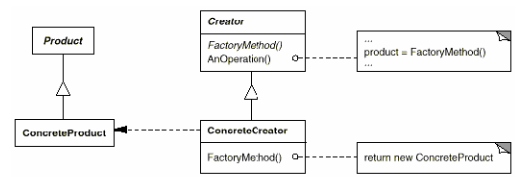
\includegraphics[width=.9\linewidth]{img/factory_method.png}
\caption{\label{fig:factory-method-class-diagram}Factory Method Class Diagram}
\end{figure}

\subsection{Prototype}
\label{sec:org2935abf}
\end{document}